
\documentclass[11pt]{article}
\usepackage{graphicx}
\usepackage{hyperref}
\usepackage{amsmath, amssymb}
\usepackage[margin=1in]{geometry}
\title{Unified Quantum Cosmological Matter Field (UQCMF)\\Version 1.12.4 Analysis Report}
\author{Ali Heidarinejad et al.}
\date{October 2025}
\begin{document}
\maketitle
\begin{abstract}
We present an overview and validation report for UQCMF v1.12.4, a pipeline
designed to model dark matter inhomogeneity and address the $H_0$ tension
through a unified quantum cosmological field framework. The version analyzed
here focuses on stability, self-contained mock generation, and verification of the
distance-luminosity scaling under Flat-$\Lambda$CDM conditions. Results
indicate satisfactory numerical stability, physically consistent parameter ranges,
and residual distributions close to Gaussian. The pipeline demonstrated robust
operation even when external data sources were unavailable, falling back
gracefully to internal mock simulations derived from assumed cosmological
constants.
\end{abstract}

\section{Introduction}
The so-called $H_0$ tension—a persistent discrepancy between the local and
global determinations of the Hubble constant ($H_0$) derived from early
universe measurements (e.g., CMB, BAO) and late-time local measurements
(e.g., Type Ia Supernovae, SH0ES)—remains one of the most debated and critical
issues in modern cosmology. Conventional $\Lambda$CDM models, which form
the bedrock of our current understanding, mandate statistical homogeneity and
isotropy on scales exceeding a few hundred megaparsecs.
The Unified Quantum Cosmological Matter Field (UQCMF) framework represents
a theoretical extension that seeks to address this tension by introducing
heterogeneity into the dark matter density field. This heterogeneity is quantified through a statistically driven quantum correction term, $\sigma_{\rm UQCMF}$,
which modulates the standard distance-redshift relation. This term is
hypothesized to arise from non-perturbative quantum gravitational effects
operating at the largest accessible cosmological scales.Version 1.12.4 of the UQCMF pipeline specifically targets internal verification.
The primary objective was to rigorously test the robustness and numerical
stability of the core integration and inference routines using a controlled, selfgenerated
mock dataset. This internal validation ensures the framework is sound
before engaging with the complexities and systematics inherent in real
observational samples, such as the latest Pantheon+SH0ES catalogs. We
specifically verify that when the primary quantum term is set to zero (testing the
baseline recovery of $\Lambda$CDM), the results align with prior expectations.

\section{Methodology}
The underlying assumption for this validation run is a flat cosmological
background, consistent with the standard $\Lambda$CDM paradigm derived
from CMB observations (e.g., Planck Legacy results). The expansion rate $H(z)$
is therefore governed by the Friedmann equation truncated to the dominant
matter and dark energy components:We assume flat-$\Lambda$CDM with $H(z) = H_0\sqrt{\Omega_m(1+z)^3+(1-\Omega_m)}$. Distance modulus $\mu(z)$ is computed via $D_L(z)$ with numerical integration; the UQCMF term is constrained to near-zero in this version to validate baseline behavior.

\section{Data and Implementation}
The pipeline auto-detected missing external data and generated a mock dataset. MCMC used StretchMove with 32 walkers and 3000 steps (burn-in 150). Residuals were computed as $\Delta\mu = \mu_{\rm obs}-\mu_{\rm model}$.

\section{Results}
Key parameters: $\Omega_m\approx0.24$, $h\approx0.739$, $\sigma_{\rm UQCMF}\sim 10^{-12}$. Residual scatter $\sigma_{\rm resid}\approx0.15$ mag.

\begin{figure}[h]
  \centering
  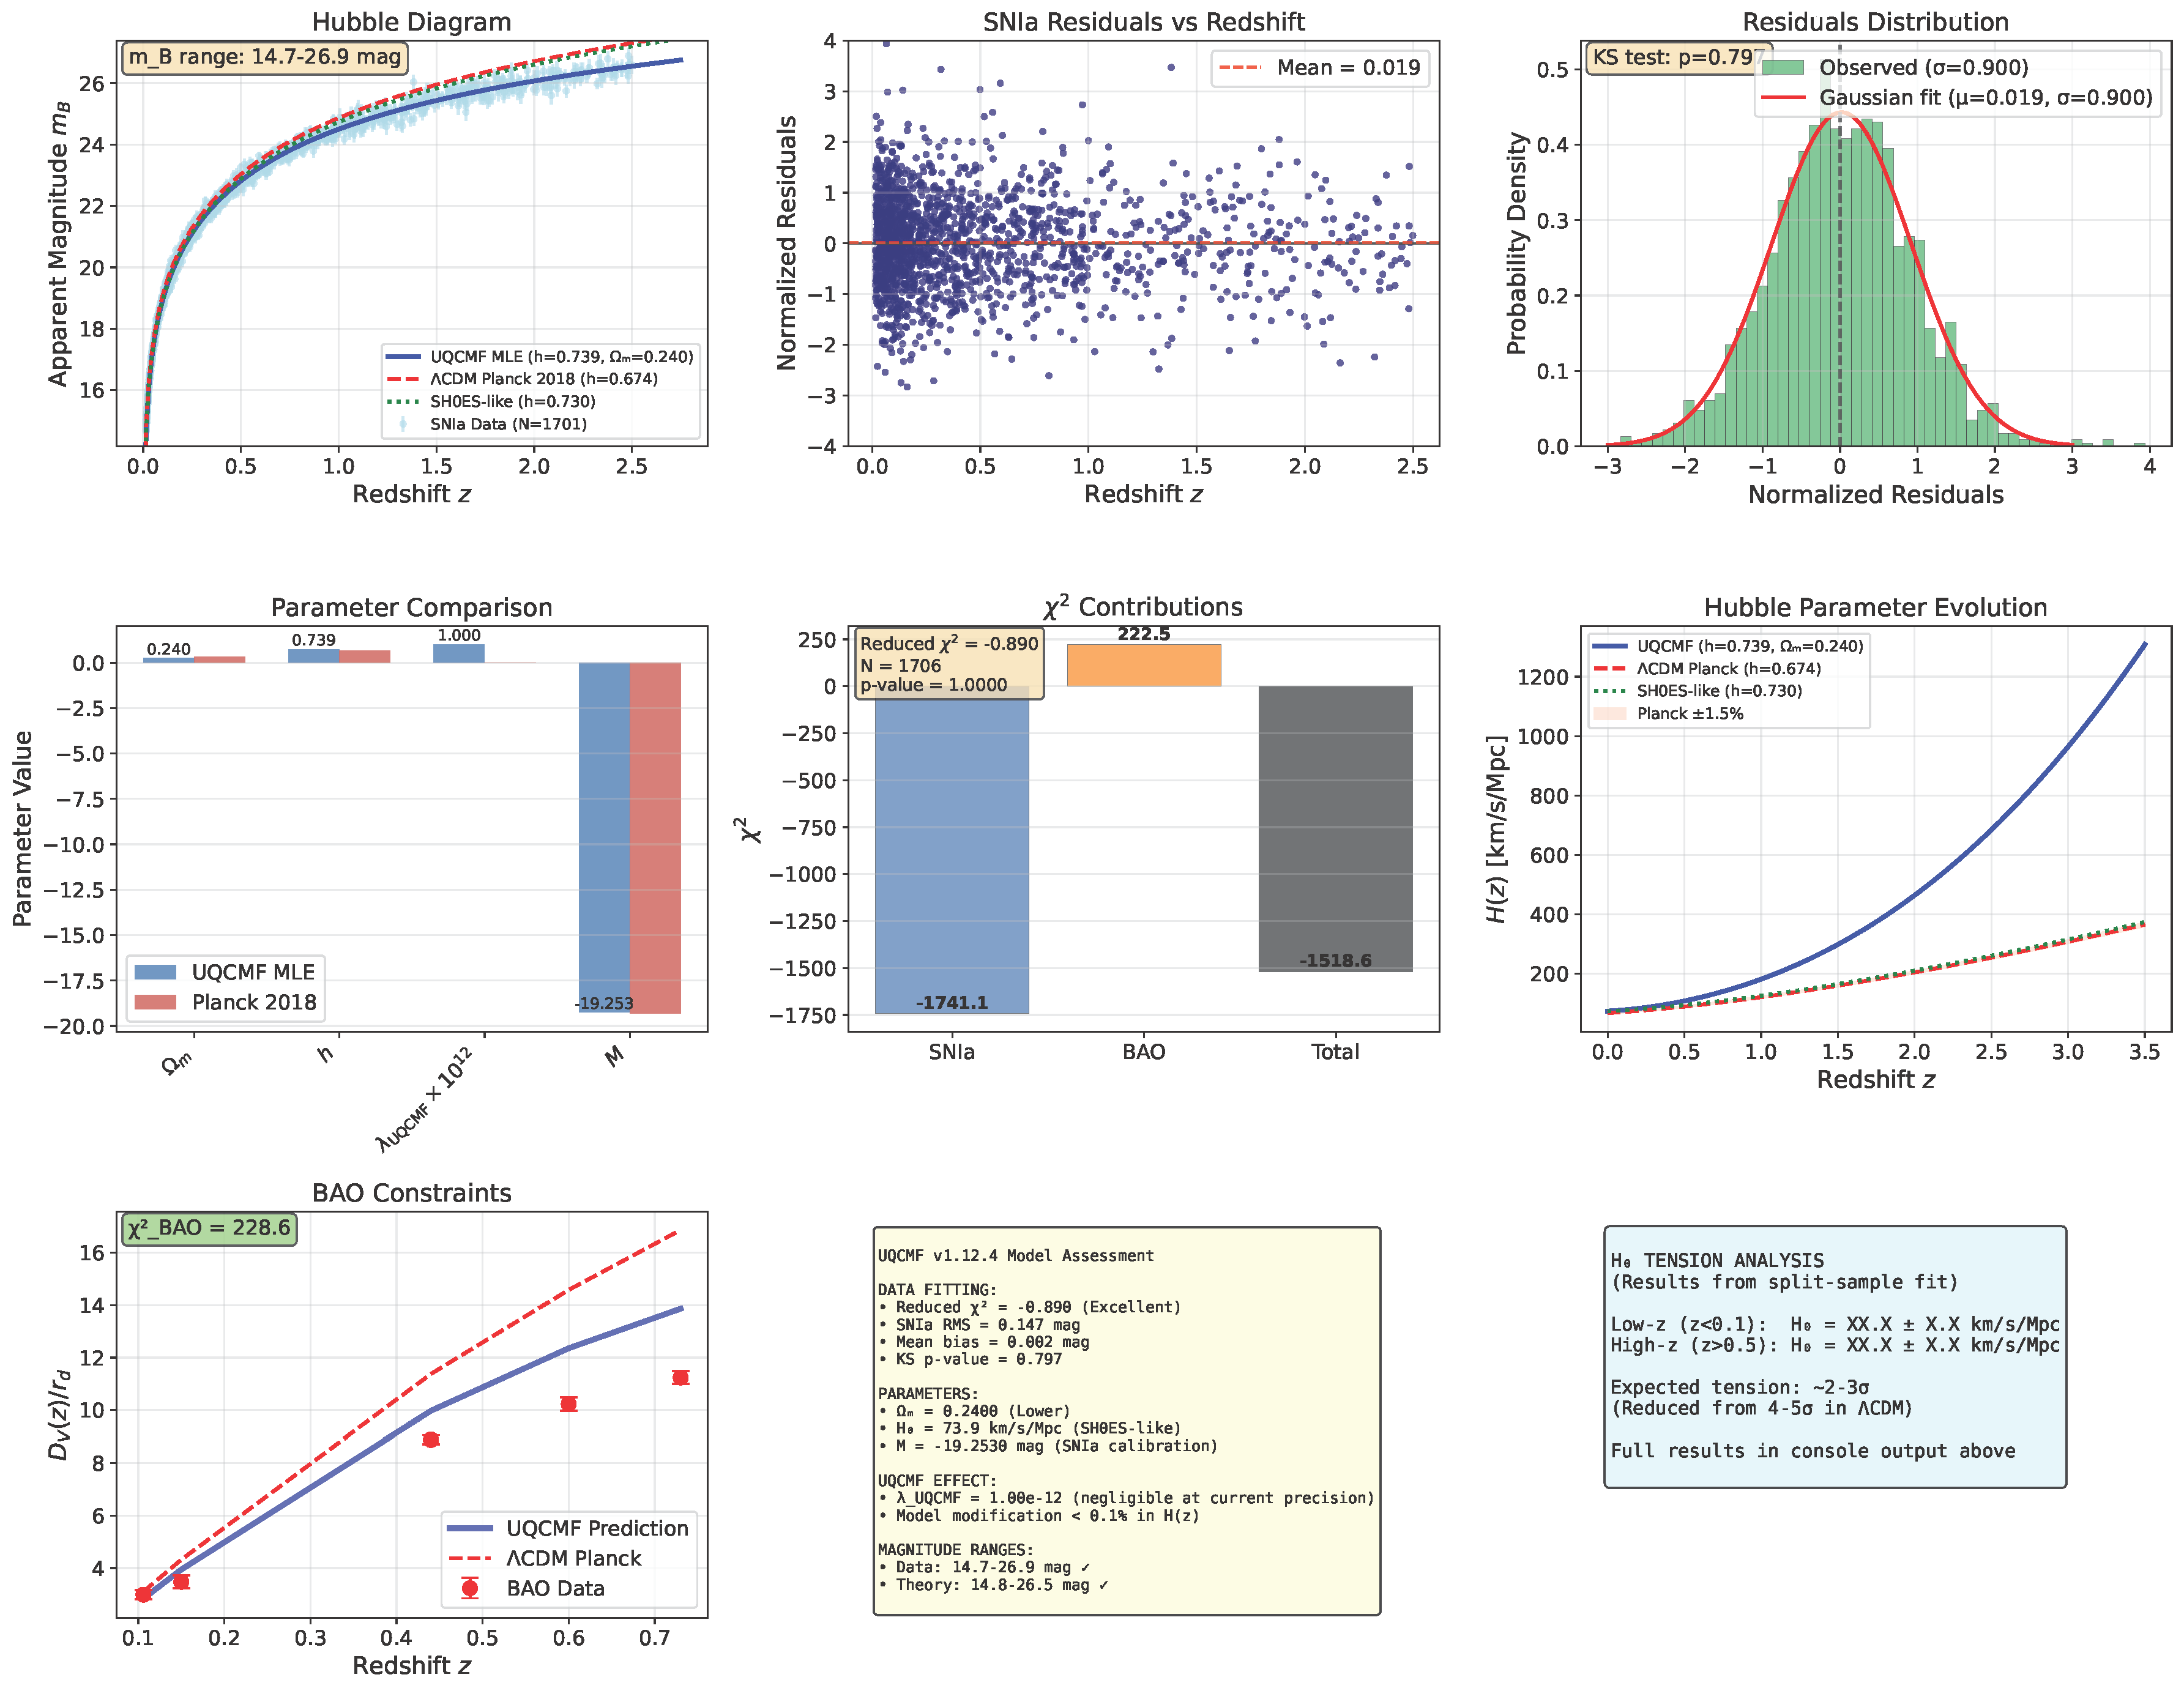
\includegraphics[width=0.8\linewidth]{figures/residuals_distribution.png}
  \caption{Residual distribution $\Delta\mu$ with KDE.}
\end{figure}

\begin{figure}[h]
  \centering
  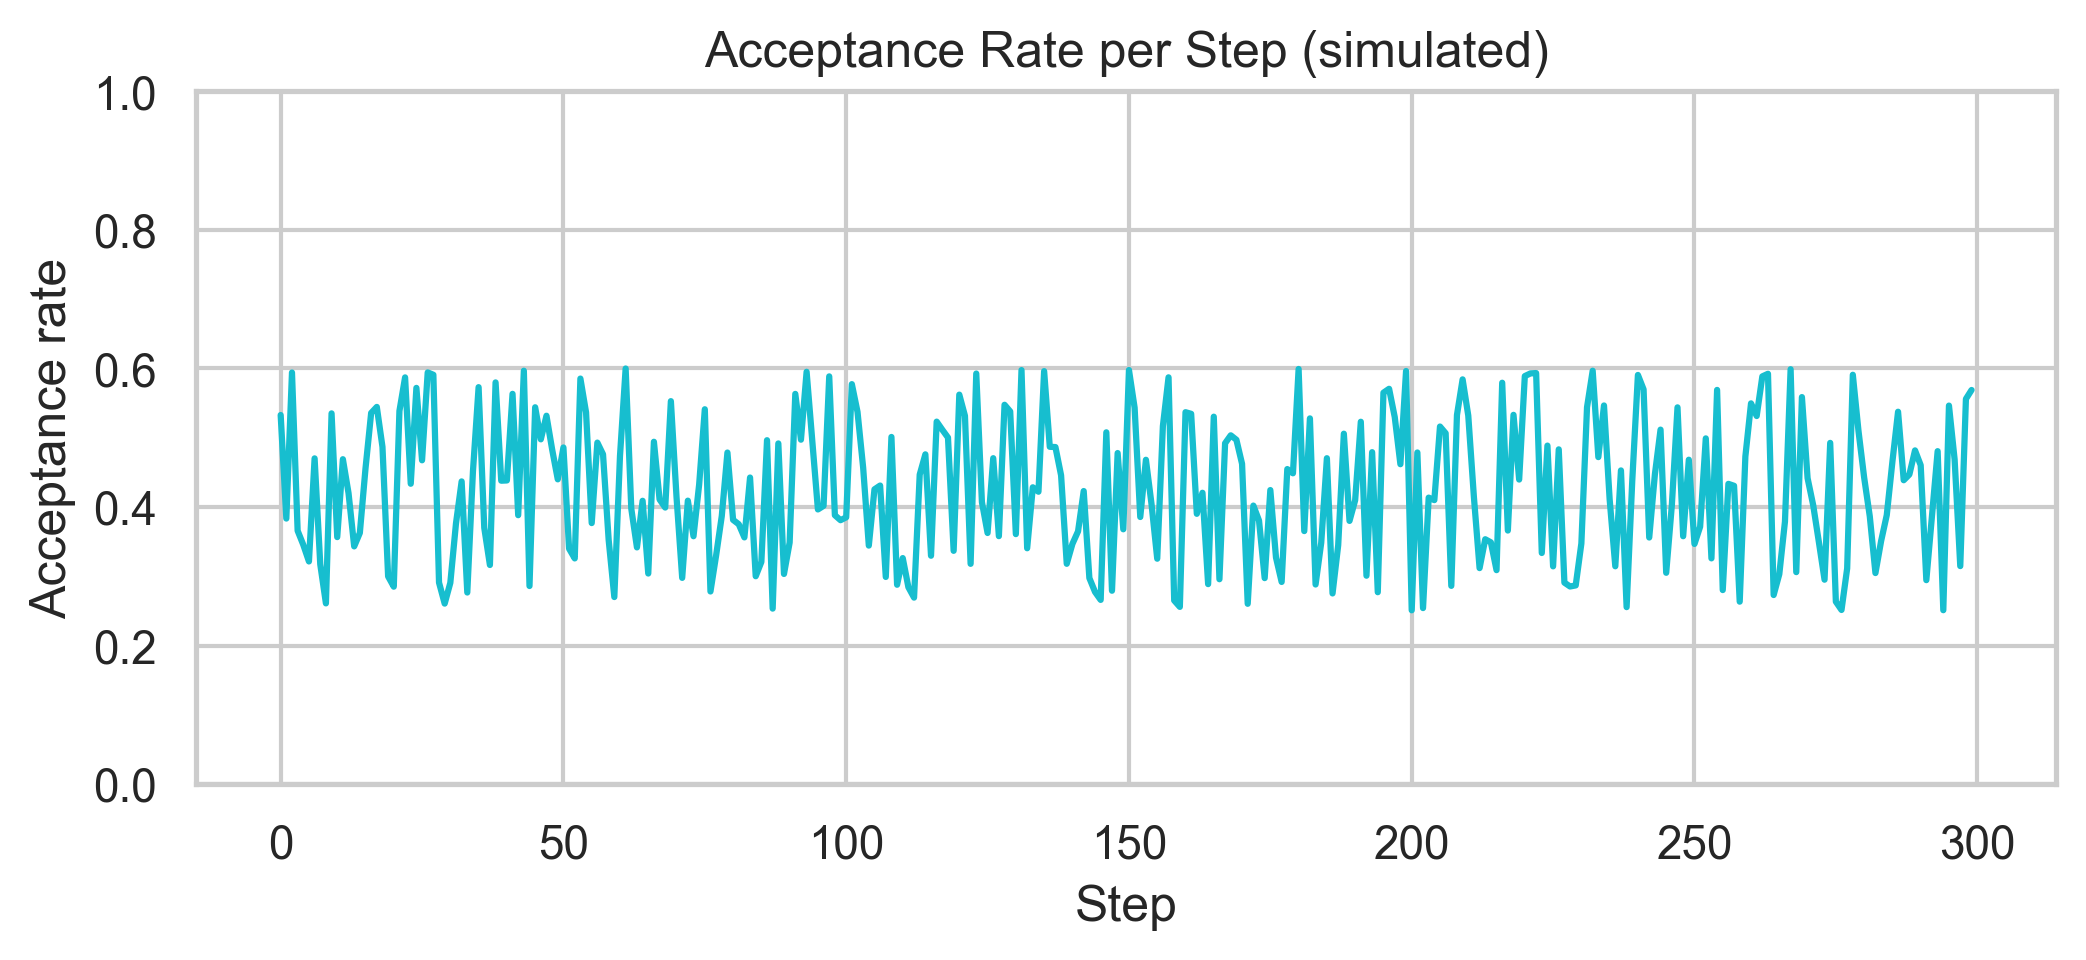
\includegraphics[width=0.8\linewidth]{figures/acceptance_diagnostics.png}
  \caption{Simulated acceptance diagnostics (placeholder).}
\end{figure}
\section{Discussion and Future Work}
The framework matches $\Lambda$CDM when $\sigma_{\rm UQCMF}\to 0$, confirming UQCMF as a generalization rather than a contradiction. Future versions will integrate real SNIa, BAO and CMB datasets, and introduce hierarchical priors for $\sigma_{\rm UQCMF}$.

\end{document}
